 \documentclass[a4paper,anonymous,USenglish]{lipics-v2019}
 
 \usepackage[utf8]{inputenc}
 \usepackage{xspace}
 \usepackage{balance}
 \usepackage{amsmath,amsfonts,mathtools,amsthm}
 \usepackage{algorithmic}
 \usepackage{algorithm}
 
 \usepackage{balance}
 \usepackage{amsthm,amsmath,array,colortbl,graphicx,multirow}
 \usepackage{comment}
 \usepackage{balance}
 \usepackage{tikz}
 \usepackage{amsmath}
 \usetikzlibrary{patterns} %
 \usepackage{algorithm}
 \usepackage[font={footnotesize}]{subcaption}
 \usepackage[font={footnotesize}]{caption}
 \usepackage{breakcites}
 \usepackage{booktabs}
 \usepackage{diagbox}
 \usepackage{xcolor}
 \usepackage{colortbl}
 \usepackage{cleveref}
 \usepackage{enumitem}
 
 \mathchardef\mhyphen="2D
 
 \title{Tight Bounds for Dynamic Balanced Graph Partitioning}
 
 \author{Maciej Pacut}{maciej.pacut@univie.ac.at}{Faculty of Computer Science, University of Vienna,Austria}{0000-0002-6379-1490}{}
 
 
 \author{Mahmoud Parham}{mahmoud.parham@univie.ac.at}{Faculty of Computer Science, University of Vienna, Austria}{0000-0002-6211-077X}{}
 
 \author{Stefan Schmid}{stefan\_schmid@univie.ac.at}{Faculty of Computer Science, University of Vienna, Austria}{}{}


 \authorrunning{M. Pacut, M. Parham, and S. Schmid}
 \Copyright{Maciej Pacut, Mahmoud Parham, and Stefan Schmid}
 \keywords{online algorithms, competitive analysis, distributed computing, graph partitioning, clustering, self-adjusting networks}
 
% \EventEditors{}
%\EventNoEds{3}
 \EventLongTitle{34th International Symposium on DIStributed Computing (DISC) 2020)}
 \EventShortTitle{DISC 2020}
 \EventAcronym{DISC}
 \EventYear{2020}
 \EventDate{October 12--16, 2020}
 \EventLocation{Freiburg, Germany (virtual conference)}
 \EventLogo{}
 \SeriesVolume{}
 \ArticleNo{}
 

 \ccsdesc[500]{Networks~Network algorithms}
 \ccsdesc[300]{Computer systems organization~Cloud computing}
 \ccsdesc[300]{Computer systems organization~Distributed architectures}
 \ccsdesc[500]{Theory of computation~Online algorithms}
 
 %%%%%%%%%%%%%%%%%%%%%%%%%%%%%%%%%%%%%%%%%%%%%%%%&&
 %%%%%%%%%%%%%%%%%%%%%%%%%%%%%%%%%%%%%%%%%%%%%%%%&&
 %  our macros start
 %%%%%%%%%%%%%%%%%%%%%%%%%%%%%%%%%%%%%%%%%%%%%%%%&&
 %%%%%%%%%%%%%%%%%%%%%%%%%%%%%%%%%%%%%%%%%%%%%%%%&&
 
 \newcommand{\OPT}{\textsf{OPT}\xspace}
  \newcommand{\OPTM}{\mathit{OPT}}
 \newcommand{\ALG}{\textsf{ALG}\xspace}
 \newcommand{\PPL}{\textsf{PPL}\xspace}
 \newcommand{\OBRP}{BRP\xspace}
 \newcommand{\PPOBRP}{PP-BRP}
 \newcommand{\dist}{\textsf{dist}}
 \newcommand{\TAlg}{{\ensuremath{\textsf{ALG}_{3}}}\xspace}
  \newcommand{\RM}{\textsf{RM}\xspace} % rematching alg
 
 \newcommand{\comm}{\textsc{comm}}
 \newcommand{\OFF}{\textsc{Off}\xspace}
 \newcommand{\Rep}{\textsc{Rep}}
 
 
 
 
 %\newtheorem{claim}{Claim}
 \newtheorem{fact}{Fact}
 \newtheorem{rem}{Remark}
 \newtheorem{observation}{Observation}
 \newtheorem{property}{Property}
 
 
 \DeclarePairedDelimiter\pair{(}{)}
 \DeclarePairedDelimiter\set{\{}{\}}
 
 \DeclarePairedDelimiter{\ceil}{\lceil}{\rceil}
 \DeclarePairedDelimiter{\floor}{\lfloor}{\rfloor}
 
 \newcommand\mahmoud[1]{\color{orange}\textbf{Mahmoud: #1~}\color{black}}
 \newcommand\stefan[1]{\color{blue}\textbf{Stefan: #1}\color{black}}
 \newcommand\maciek[1]{\color{brown}\textbf{(Maciek: #1)}\color{black}}
 %\newcommand\mahmoud[1]{}
 %\newcommand\stefan[1]{}
 %\newcommand\maciek[1]{}
 
 
 \newcommand{\todo}[1]{\noindent\color{brown}{todo: #1}\color{black}}
 
 \begin{CCSXML}
	<ccs2012>
	<concept>
	<concept_id>10003033.10003068</concept_id>
	<concept_desc>Networks~Network algorithms</concept_desc>
	<concept_significance>500</concept_significance>
	</concept>
	<concept>
	<concept_id>10010520.10010521.10010537.10003100</concept_id>
	<concept_desc>Computer systems organization~Cloud computing</concept_desc>
	<concept_significance>300</concept_significance>
	</concept>
	<concept>
	<concept_id>10010520.10010521.10010537</concept_id>
	<concept_desc>Computer systems organization~Distributed architectures</concept_desc>
	<concept_significance>300</concept_significance>
	</concept>
	</ccs2012>
\end{CCSXML}

% for my small screen
%\setlength{\textwidth}{8cm}

\begin{document}

\begin{abstract}
	Distributed   applications,  including  batch  processing, streaming, scale-out databases,
	or machine learning, generate a significant amount of network traffic.
	By collocating frequently communicating nodes (e.g., virtual machines) on the same clusters (e.g., server or rack), we can reduce the network load and  improve application performance. 
	However, the communication pattern of different application is often unknown a priori, and may change over time, hence it needs to be learned in an online manner.
	%
	This paper revisits the online 
	balanced repartitioning problem 
	(introduced by Avin et al.~at DISC 2016)
	which asks for an algorithm that strikes
	an optimal tradeoff between the benefits
	of collocation (i.e., lower network load) 
	and its costs (i.e., migrations). 
	%
	Our first contribution is a significantly improved
	lower bound of $\Omega(k\cdot \ell)$ on the
	competitive ratio, where $\ell$ is the number
	of clusters and $k$ is the cluster size,
	even for a scenario in which the communication
	pattern is static and can be perfectly partitioned;
	we also provide a \mahmoud{asymptotically?} tight upper bound 
	of $O(k\cdot \ell)$ for this scenario.
	We contribute a tight upper bound
	of $\Theta(\ell)$ for $k=3$,
	for the general model in which the
	communication pattern can change arbitrarily
	over time.
	We improve the result for $k=2$ by providing a strictly $6$-competitive upper bound for the general model.
	In contrast to most prior work, our algorithms respect all capacity constraints, and do not require resource augmentation.
	
\end{abstract}

\maketitle

%\renewcommand{\shortauthors}{M.~Pacut, M.~Parham, S.~Schmid}


\section{Introduction}


The popularity of data-centric, distributed applications has led to an explosive growth of network traffic, especially in data centers \cite{roy2015inside,singh2015jupiter}.
As the performance of these distributed applications often critically depends on the underlying network \cite{mogul2012we}, an efficient operation of these networks is important.
At the same time, distributed systems are often highly virtualized today, and provide interesting new opportunities for resource optimization.
In particular, it has become possible to operate data centers in a more demand-aware manner: 
by dynamically migrating nodes (e.g., virtual machines) which communicate frequently topologically closer to each other, network traffic can be reduced significantly.  
However, migrations should be used moderately, as migrations also entail overheads. 

This paper studies the algorithmic problem underlying such demand-aware
optimizations, aiming to strike a balance between the benefits of migrations (e.g., reduced network load) and their costs.
In particular, we are interested in an online variant of the problem: since communication patterns can change over time, an online algorithm needs to react dynamically to new traffic patterns, and migrate nodes  accordingly.
Ideally, this algorithm should perform close to an optimal offline algorithm, without requiring any information about future traffic demands. 

This problem is known as the dynamic balanced graph partitioning problem introduced by Avin et al. \cite{repartition-disc, sidma-arxiv} at DISC 2016. A special variant of the general problem has later been studied by Henzinger et al. \cite{sigmetrics19_partitioning} at SIGMETRICS 2019.
We will refer to the latter as the learning model.



\subsection{Model}

We study two models in this paper: the \emph{general partitioning} model, and its subproblem, the \emph{learning} model.

\noindent
\textbf{General partitioning model.}
In the \emph{dynamic balanced graph partitioning} problem, we are given a set $V$ of $n$ nodes 
(e.g., virtual machines or processes),
initially arbitrarily partitioned into $\ell$~clusters
(e.g., servers or entire racks),
each of size~$k$.
The nodes interact using
a~sequence of pairwise communication requests
$\sigma = (u_1,v_1),$ $(u_2,v_2),$ $(u_3,v_3), \ldots$,
where a pair $(u_t,v_t)$ indicates that nodes $u_t$ and $v_t$ exchange a~certain amount of data.
Nodes in $C \subset V$ are \emph{collocated}
if they reside in the same cluster.

An algorithm serves a communication request between two nodes
either \emph{locally} at cost~0
if they are collocated,
or \emph{remotely} at cost~1
if they are located in different clusters.
We refer to these two types of requests as \emph{internal}
and \emph{external} requests, respectively.
Before serving a request,
an online algorithm may perform a \emph{repartition},
%(i.e., \emph{reconfigure}).
i.e.,
it may move (``migrate'') some nodes into clusters different from their current clusters, while respecting the capacity of every cluster. 
Afterwards, 
the algorithm serves the  request.
The cost of migrating a node from one cluster to another
is~$\alpha \in \mathbb{Z}^+$.
For any algorithm $\ALG$,
its cost,
denoted by $\ALG(\sigma)$,
is the total cost of communications and
the cost of migrations performed by $\ALG$ while serving the sequence $\sigma$.



\noindent
\textbf{Learning model.}
We study a variant of Online Balanced Partitioning,
where the communication pattern is \emph{static}:
an adversary determines the pairs of nodes that ever communicate, a~priori,
and requests to these pairs arrive indefinitely.
Any algorithm must eventually collocate  pairs of communicating nodes,
as otherwise it cannot be competitive.
As in Henzinger et al. \cite{sigmetrics19_partitioning}, we assume that the communication graph admits a \emph{perfect partition},
i.e., a partition in which no inter-cluster request ever occurs.
%any algorithm must learn this perfect partition.
The algorithm's objective is to \emph{learn} the (static) communication graph
 while serving all requests,
and without executing too many migrations.
For the learning model, we  assume that the migration cost is $\alpha=1$.

\medskip 
In both models, we assume that communication patterns are not known to our algorithms at the beginning.
We measure the~quality of~presented algorithmic solutions by competitive analysis~\cite{borodin-book}, which is well-suited for problems that are online by their nature.
In the competitive analysis, the goal is to~optimize \emph{the competitive ratio} of a given online algorithm: the ratio of its cost to the cost of~an~optimal offline algorithm that knows the whole input sequence in advance.


\subsection{Related work}

The two works closest to ours are by Avin et al. (on the general partitioning model) \cite{repartition-disc, sidma-arxiv} and by Henzinger et al. (on the learning model) \cite{sigmetrics19_partitioning}.
The focus of these papers however is primarily on models with resource augmentation: the online algorithm can use slightly larger clusters than the offline algorithm.  
Avin et al. actually showed that their lower bound $\Omega(k)$ holds even for a significant resource augmentation, and they provided an algorithm with the competitive ratio $O(k \log k)$ using the $(2+\epsilon)$-augmented cluster capacity.
Their ratio is independent of $\ell$, which is impossible without significant resource augmentation.



In contrast, we study the non-augmented setting, where the nodes need to be perfectly balanced  among the clusters.
This assumption is not only more realistic but also significantly more challenging, as it is related to hard problems such as integer partitioning \cite{integer-partitions-book}.
In terms of results without augmentation, so far, it is only known that there exists a $O(k^2 \cdot \ell^2)$-competitive algorithm \cite{repartition-disc}; the best known lower bound is significantly lower, namely $\Omega(k)$.
For $k=2$, Avin et al.\cite{repartition-disc} presented a $7$-competitive algorithm with a~substantial ($\Omega(\ell^2)$) additive constant.


The problem has also been studied in a weaker
model where the adversary can only sample
requests from a fixed distribution~\cite{stochastic-ring}.

The static offline version of~the~partitioning~problem, i.e., a problem variant where
migration is not allowed, where all requests are known in advance, and where
the goal is to find an assignment of $n$ nodes to $\ell$~physical machines, each of~capacity $n/\ell$, is known as the
\emph{$\ell$-balanced graph partitioning problem}. The problem is 
NP-complete, and cannot even be approximated within any finite factor unless P
= NP~\cite{AndRae06}.  The static
variant where $\ell = 2$ corresponds to the minimum bisection problem, which
is already NP-hard~\cite{GaJoSt76}, and 
the currently best approximation ratio is $O(\log n)$~\cite{SarVaz95,ArKaKa99,FeKrNi00,FeiKra02,KraFei06,Raec08}.

Our problem is further related to some classic online problems.
In particular, it is related to online paging~\cite{SleTar85,FKLMSY91,McGSle91,AcChNo00}, sometimes also referred to
as online caching, where requests for data items (nodes) arrive over time and
need to be served from a cache of finite capacity, and where the number of
cache misses must be minimized. Classic problem variants usually boil down to
finding a smart eviction strategy, such as Least Recently Used (LRU)~\cite{SleTar85}. In our
setting, requests can be served remotely (i.e.,~without fetching the
corresponding nodes to a single physical machine). In this light, our model is more
reminiscent of caching models \emph{with
bypassing}~\cite{EpImLN11,EpImLN15,Irani02}.
A major difference between  these problems is that in the caching problems, each request involves a~single element of the universe, while in our model \emph{both} endpoints of a communication request are subject to~optimization.
In this light, we can see our model as a "symmetric" version of online paging.

Dynamic graph partitioning problems are generally fundamental in computer science, and arise in many different contexts \cite{streaming-soda,streaming1}.

%More generally, the model is related to online
%caching~\cite{SleTar85,FKLMSY91,McGSle91,AcChNo00},
%see~\cite{repartition-disc} for a discussion.
%The static offline version of~the~problem, called the
%\emph{$\ell$-balanced graph partitioning problem} is 
%NP-complete, and cannot even be approximated within %any finite factor unless P
%= NP~\cite{AndRae06}. 

\subsection{Our Contributions}

This paper presents several new results on the dynamic graph partitioning problem  without augmentation.
Our main result is a tight bound on the general case: we present a lower bound of $\Omega(k\cdot\ell)$ on the competitive ratio of any online deterministic online algorithm 
even in the learning model.
The best known lower bound so far was $\Omega(k)$,
even for a more general model~\cite{repartition-disc}.
We also present an asymptotically optimal, 
$O(k\cdot \ell)$-competitive algorithm
for the learning model.
For the repartitioning model, we present  
an asymptotically optimal,
$\Theta(\ell)$ algorithm for $k=3$, improving the best known upper bound 
so far $O(\ell^2)$~\cite{repartition-disc}.
We further present a strictly $6$-competitive algorithm for $k=2$ that improves upon previous $7$-competitive algorithm with $O(\ell^2)$ additive constant.
%
Table \ref{tab:overview} provides an overview of our contributions compared to prior work.

\begin{table*}
	\centering
	\renewcommand{\arraystretch}{1.5}
	\begin{tabular}{>{\centering\arraybackslash}p{4.5cm}|>{\centering\arraybackslash}p{4.5cm}>{\centering\arraybackslash}p{4.5cm}}
		\rowcolor{gray!50}
		\textbf{Variant} & \textbf{ Lower bound} &\textbf{Upper bound}\\ \hline 
		\textbf{$k=2$}& 3\hspace{0.3cm}\cite{repartition-disc} & 6\hspace{0.3cm}(\S \ref{sec:k2}) \\ 
		\rowcolor{gray!25}
		\textbf{$k=3$}&  $\Omega(\ell)$ \hspace{0.3cm}(\S \ref{sec:lowerbound})& $O(\ell) $\hspace{0.3cm}(\S \ref{sec:k3})\\
		$k > 3$ & $\Omega(k\cdot \ell)$\hspace{0.3cm}(\S  \ref{sec:lowerbound})&$O(k^2 \cdot \ell^2)$\hspace{0.1cm} \cite{repartition-disc} \\
		\rowcolor{gray!25}
		Learning model & $\Omega(k\cdot \ell)$\hspace{0.3cm}(\S  \ref{sec:lowerbound})&$O(k \cdot \ell)$\hspace{0.3cm} (\S \ref{sec:ppl}) \\
	\end{tabular}
	\caption{Overview of known results and the results provided in this paper. By $\Rep$ we denote the cost of a single component repartition, and we elaborate on this in Section~\ref{sec:k3}. The first three rows show the results for the general partitioning model, except for the last row that shows the results for the learning model for arbitrary $k$ and $\ell$.
	}
	\label{tab:overview}
	\vspace{-7mm}
\end{table*}

\section{The Learning Problem} %$\Omega(k\cdot \ell)$ for Competitive Ratio of Any Deterministic Algorithm}

In this section we consider the learning variant of Dynamic Balanced Graph Partitioning.
For this setting, we show a surprisingly high lower bound of $\Omega(k \cdot \ell)$.
The lower bound can be easily translated to the partitioning model (studied in Section~\ref{sec:part}) with finite request sequence.
At the end of this section, we discuss an asymptotically optimal upper bound.


\subsection{Lower Bound}

\label{sec:lowerbound}


We provide a lower bound $\Omega(k\cdot \ell)$ for the competitive ratio of any deterministic online algorithm for the learning problem.
Later we elaborate on how to efficiently transform it to a lower bound for the general partitioning problem.
The lower bound requires $k\geq 3$.
For $k=2$, the learning problem is trivial: immediate collocation of a communicating pair is $1$-competitive.
(A partitioning problem for $k=2$ is non-trivial, a lower bound of $3$ is known \cite{repartition-disc}, and we provide a~$6$-competitive algorithm (see Section~\ref{sec:k2}).)




\begin{figure}[H]
	\centering
	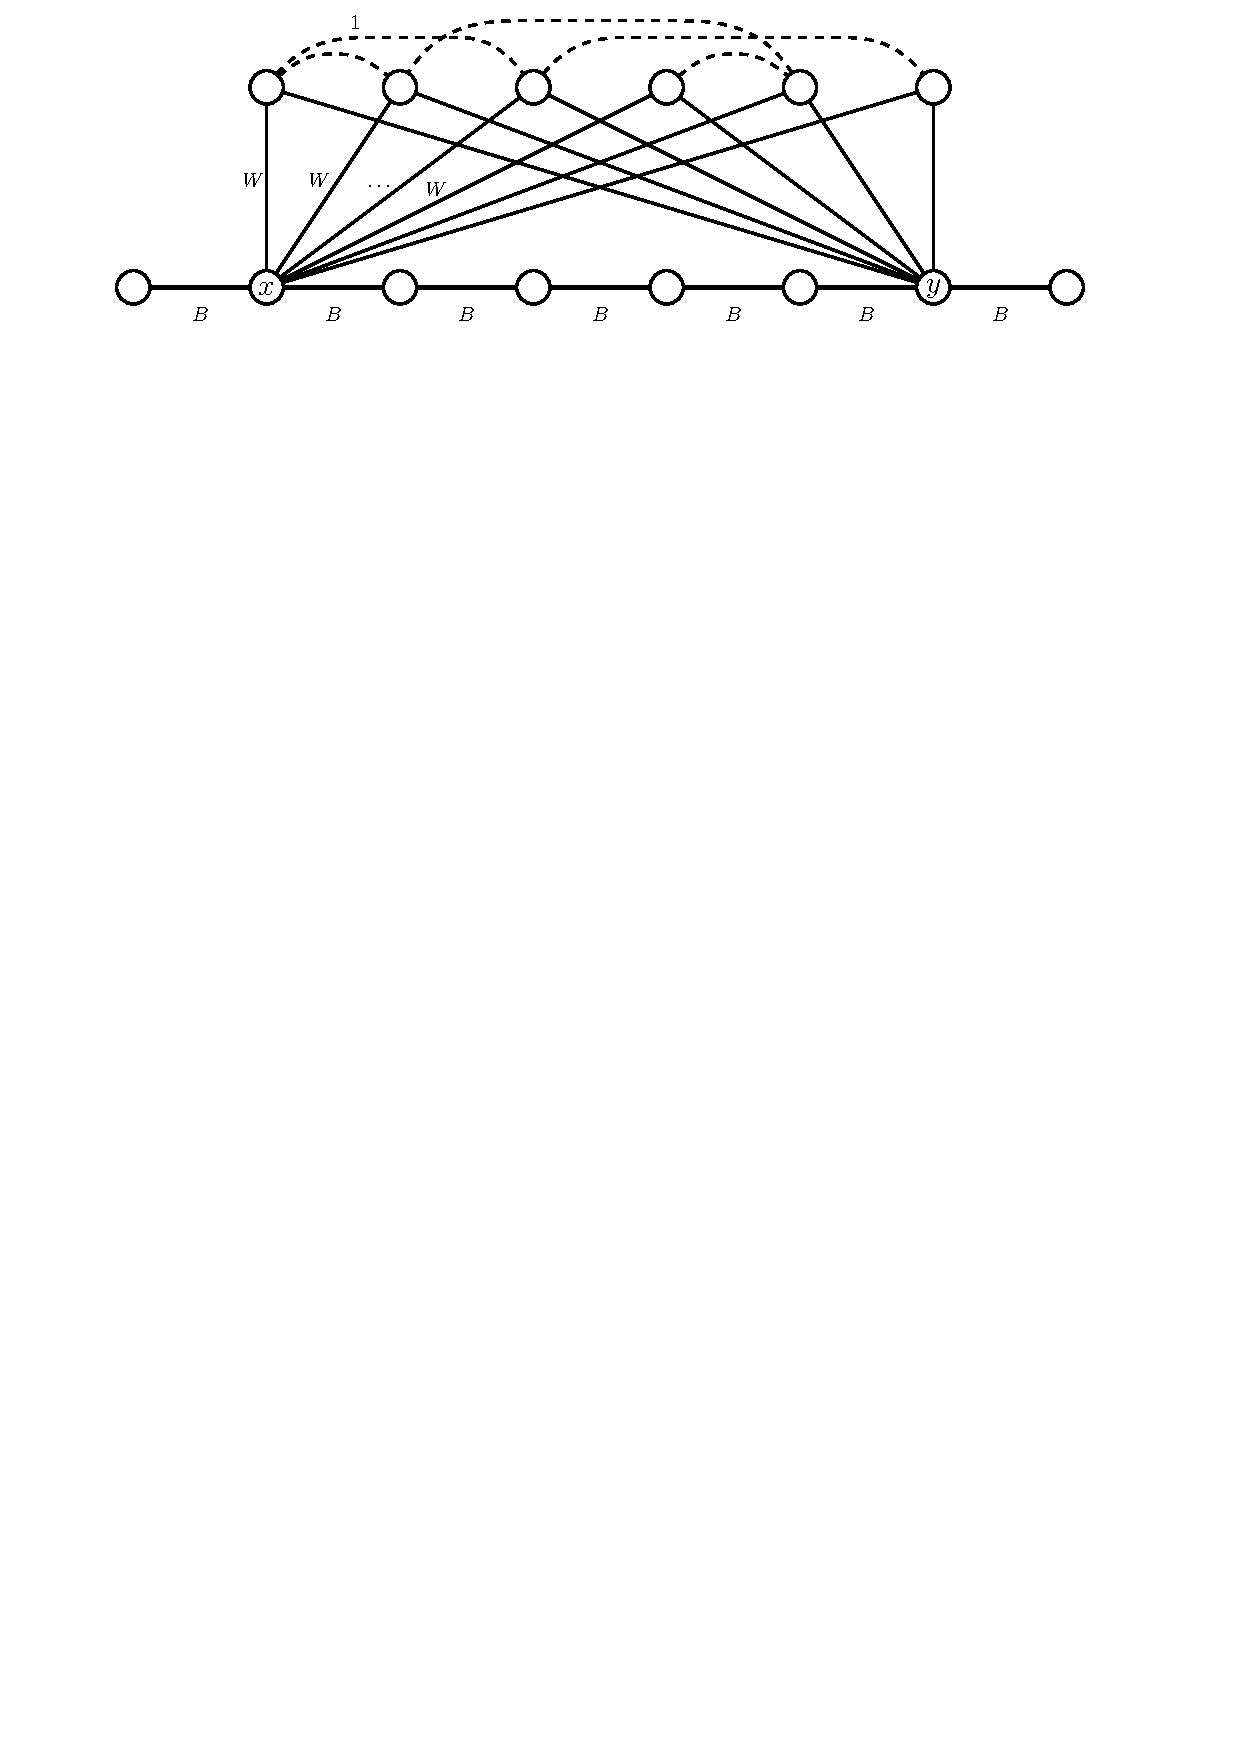
\includegraphics[width=0.3\textwidth]{figs/substitute}
	\caption{Example figure of the construction of the LB and growing components.}
	\label{fig:nptree-construction}
\end{figure}


Across this paper, we often refer to groups of communicating nodes.
We use this concept slightly differently in the lower bound and the upper bounds.
In our algorithms, we group nodes with a communication history into \emph{components}, and in the lower bound, we group nodes that may communicate into \emph{ground sets}.


A~\emph{ground set} is a group of nodes that repeatedly communicate when an algorithm splits them (places at different clusters).
Their role is to ensure that the algorithm maintains a~partition of ground sets into clusters.
We emphasize that ground sets are revealed only upon their nodes are split.
We say that a ground set is \emph{trivial}, if it contains exactly one node.
We say that the node that belongs to trivial a ground set is \emph{isolated}.


The adversary constructs ground sets depending on choices of a deterministic online algorithm.
We emphasize that the algorithm does not know ground sets before they are revealed.
Once we construct a ground set, it lasts until the end of the input sequence.

The constructed ground sets can be perfectly partitioned into the clusters (i.e., with nodes of each ground set collocated).
This way, the optimal algorithm moves to a perfect partition at the beginning (where requests incur the cost~$0$), thus its cost is bounded.
If the algorithm splits any pair of nodes of a ground set, the adversary issues requests to any pair of split nodes.
These two observations imply that the algorithm must eventually collocate all nodes of a~ground set to be competitive.

First, we construct a ground set of size $k-1$ on an arbitrary cluster $S$.
In any configuration, there exists an isolated node on $S$.
We issue requests between the current isolated node from $S$, and some node that was initially collocated with it.
Repeating such requests, almost all the nodes must visit the cluster $S$.
In comparison, \OPT performs only two migrations.

\begin{theorem}
	\label{th:lowerbound}
	The competitive ratio of any deterministic online algorithm for the learning model of Dynamic Balanced Graph Partitioning is at least $(k\cdot \ell - k - \ell)/2$ for any $k\geq 3$ and $\ell \geq 2$.
\end{theorem}

\begin{proof}
	Fix any online algorithm \ALG{}.
	Let $I(C)$ denote the cluster where nodes of the ground set $C$ are located in the initial configuration.
	If $C$ contains nodes that originate from different clusters, $I(C)$ is undefined.
	Throughout the construction, we maintain ground sets for each node.
	Initially all nodes are \emph{isolated}.
	First, we create a ground set $B$ of $k-1$ nodes on an arbitrarily chosen cluster (the nodes  are already collocated).
	%We never dismiss any constructed ground set.
	Each cluster hosts exactly $k$ nodes, and in any configuration a single isolated node resides in $S$.
	We say that this isolated node that accompanies the ground set $B$ is \emph{special}.
	We denote the first special node by $x_0$.

	Then, we add the special node to a larger ground set to force its eviction.
	Precisely,
	we create a ground set $\{x_0, y_0\}$, 
	where $x_0$ is the current special node and $y_0$ is an arbitrary node that does not reside in $S$.
	\ALG has them split, and the adversary issues external requests until \ALG collocates them.
	There is no space to accommodate $\{x_0, y_0\}$ in the cluster of $x_0$ (as $B$'s size is $k-1$), hence \ALG must collocate $\{x_0, y_0\}$ in another cluster.
	To preserve a feasible partition of nodes into clusters after collocating $\{x_0, y_0\}$,
	\ALG must replace $x_0$ with another single node that we call $x_1$.

	We continue adding the current special node to a larger ground set.
	Precisely, for an isolated node $x_i$ from~$S$, we merge the ground sets of $x_i$ and the largest ground set $C$ s.t. $C \neq \{x_0,y_0\}$ and $I(C) = I(x_i)$.
	This way, $x_i$ is evicted similarly to $x_0$, and we continue creating such ground sets.
	We describe the termination condition shortly.
	(Note that these ground sets contain nodes that originate from the same cluster, whereas the nodes $x_0$ and $y_0$ originate from distinct clusters.)

	We claim that expanding ground sets in this way can continue as long as at least $\ell$ isolated nodes exists.
	Fix the configuration just before the creation of a ground set with $x_i$ for some $i$.
	We show that if at least $\ell$ isolated nodes exist (including $x_i$), then there exists a~perfect partition of ground sets after expanding a ground set with $x_i$.
	To show this claim, we consider a configuration, where the largest ground set of each cluster originates from it (excluding the ground set $\{x_0, y_0\}$).
	In this configuration, each cluster contains:  at most one ground set larger than $1$, possibly some isolated nodes, and possibly the ground set $\{x_0, y_0\}$.
	If $I(x_i)$ contains an isolated node, then we simply obtain a~perfect partition by swapping it with $x_i$.
	In the following we assume that no isolated nodes exist on $I(x_i)$.
	The largest ground set of $I(x_i)$ is at most $k-1$, because $x_i$ is on $S$.
	Therefore $\{x_0, y_0\}$ is present on $I(x_i)$, and we must evict it to make space for $x_i$.
	To find the cluster for $\{x_0, y_0\}$, observe that we have at most $\ell-1$ clusters with isolated nodes, and we have at least $\ell$ isolated nodes --- hence a~cluster with two isolated nodes exists.
	To find a feasible partition, we swap $\{x_0, y_0\}$ with these two collocated isolated nodes, and then we swap an isolated node from $I(x_i)$ with $x_i$.
	

	To keep \OPT's cost low, we end extending ground sets prematurely --- while there are still $\ell+1$ isolated nodes (i.e., neglecting two last ground set expansions).
	Consider \ALG's configuration after the last expansion.
	Among $\ell+1$ isolated nodes there must exist a pair that originates from the same cluster (we have $\ell$ clusters). 
	We denote these two nodes by $x^*$ and $y^*$.

	The optimal strategy is to perform two node swaps.
	Precisely, \OPT collocates $\set{x_0,y_0}$ by swapping them with $x^*$ and $y^*$.
	In this configuration, no ground set is split.
	We never issue requests between nodes $x^*, y^*$ that are split in this configuration.


	\ALG performs at least one swap for every expansion of a ground set.
	Each expansion reduces the number of isolated nodes by $1$.
	We start with $k \cdot \ell - (k-1)$ isolated nodes (a~single $k-1$ ground set is revealed prior to $\{x_0, y_0\}$), and we end with isolated $\ell+1$ nodes.
	The competitive ratio is then $\ALG / \OPT \geq (k\cdot \ell - k - l) / 2$.
\end{proof}


\noindent
\textbf{General partitioning problem.}
Every lower bound for the learning problem constitutes a converging lower bound for the partitioning problem as the input sequence grows to infinity.
However, our construction allows for an exact lower bound for partitioning with finite input sequence.
To this end, we issue only enough requests until the algorithm collocates the nodes of each ground set (if it never does, we terminate after it pays $k\cdot \ell$).
The construction is oblivious to the choice of the reconfiguration cost $\alpha$: we compare the 	number of node exchanges of \ALG and \OPT.



\noindent
\textbf{Resource augmentation.}
The majority of work on Online Balanced Partitioning so far \cite{repartition-disc,sigmetrics19_partitioning} focuses on the scenario with resource augmentation, where the clusters of \ALG are larger than the clusters of \OPT.
We can adjust our construction to show a lower bound of $\Omega(\ell)$ for resource augmentation.

Consider a partitioning problem with resource augmentation $1+1/3-\epsilon$.
Fix $k$ divisible by $3$, and construct $3$ ground sets of size $k/3$ in each cluster.
Note that no more than $3$ such ground sets fit in one cluster.
Then, apply the construction from the lower bound for $k=3$, using these ground sets in the way we used individual nodes.
The cost of any algorithm (including \OPT) scales up by $k/3$, and the lower bound $\Omega(\ell)$ holds.

Finally, we note the possibility for improvement. The algorithm CREP~\cite{repartition-disc} requires $(2+\epsilon)$-augmentation to guarantee the competitive ratio independent of $\ell$.

\subsection{Upper Bound}
\label{sec:ppl}

We present an asymptotically optimal algorithm for the learning problem.
The algorithm immediately collocates every communicating pair and never separates them.
To help maintain the collocation of communicating pairs, we use the concept of components, introduced by Avin et al. \cite{repartition-disc}.

In our algorithms, a~\emph{component} is a subset of frequently communicating nodes.
We maintain all nodes of each component collocated in one cluster~\cite{repartition-disc}.
If we need to move a~node, we move the whole component that contains it.
We maintain a balanced partition of our components, a similar concept to partition of integers into sets with equal sum \cite{integer-partitions-book}.
In contrast, our partition is time-varying: communicating components are merged into one, and we adjust the partition.

We say that a component is \emph{trivial}, if it contains exactly one node.
We say that the node that belongs to trivial component \emph{isolated}.
We say that a~configuration is \emph{component-respecting}
if the nodes belonging to the same component are collocated.

The algorithm in this section, and the algorithm for $k=3$ (cf. Section~\ref{sec:k3}) are modified versions of the algorithm DET from \cite{repartition-disc}.
The difference is in the the choice of partition after a component merge.
In DET, the partition was arbitrary.
In the algorithm for the learning model, we choose the partition closest to the initial configuration.
In the algorithm from Section~\ref{sec:k3}, we choose the partition closest to the previous configuration (a repartition of minimum cost).



\maciek{The remainder of the paper used "configuration C" to denote the partition P. Easiest to adjust here.}

\noindent
\textbf{Perfect Partition Learner algorithm.}
Fix the initial configuration
$P_I = I_1, \dots, I_{\ell}$ and \OPT's final configuration
$P_F = F_1, \dots, F_{\ell}$\maciek{How do we define a configuration?}.
The \emph{distance} of a configuration $P = C_1, \dots, C_{\ell}$ from the initial configuration \maciek{, denoted $\dist(P)$} is the number of nodes in $P$ that do not reside in their initial cluster.
\maciek{We might denote distance $\Delta(P)$, and the current $\Delta$ might be R (like radius).}
That is,
$\dist(P, P_I) := \sum_{j=1}^{\ell} | C_j \setminus I_j |$
\maciek{Major: what does this definition mean? This is highly unclear, most likely because a configuration was not defined.}. 
In other words,
at least $\dist(P, P_I)/2$ node swaps are required in order to reach the configuration $P$ from $P_I$, and thus
$\OPT \geq \Delta:= \dist(P_F, P_I) $.
With each repartitioning,
\PPL moves to a configuration that minimizes the distance to the initial configuration $P_I$.
As a result,
\PPL never ends up \maciek{ends up is informal} in a configuration that is more than $\Delta$ (single-node) migrations away from $P_I$ \maciek{This is not an algorithm definition, that's its property. Should not be in this paragraph}.
This invariant ensures that \PPL does not pay too much while recovering $P_F$ \maciek{Recovering $P_F$? It's not the goal. At least at this point the reader is confused: it does not know yet that PPL is proven to end up in $P_F$}.
%      \maciek{``re-partition'' procedure name should indicate the fact that this is a specific repartition that is close to initial partition}
We note \maciek{Define?} that the $\mathit{repartition}$ at Line \ref{line:rebalance} replaces the current configuration $P$ with a~perfect partition closest to $P_I$.
Hence it never moves to a configuration beyond distance $\Delta$ \maciek{This is again mixing the properties of ppl and its definition. Restructure}.
The scheme of the algorithm can be found in the Algorithm \ref{alg:PPL}.

\label{alg:PPL}
\begin{algorithm}
	\renewcommand{\algorithmicrequire}{\textbf{Input:}}
	\renewcommand{\algorithmicensure}{\textbf{Output:}}
	\begin{algorithmic}
		%        \Require 
		%        $k, \ell$,
		%        initial configuration $P_I$,
		%        sequence of  requests $\sigma_1, \dots, \sigma_N$ 
		%        \Ensure A final configuration $P_F$ 
		\STATE {For each node $v$ create a singleton component $C_v$ and add it to $\mathcal{C}$}
		\STATE{$P_0 := P_I$}
		\label{line:initcomponents}
		\FOR {each  request $\sigma_t=\{u,v\}, 1 \leq t \leq N$}
		\STATE Let $C_1 \ni u$ and $C_2 \ni v$ be the container components
		\IF{$C_1 \neq C_2$}
		\STATE {Unite the two components into a single component $C'$ and
		$\mathcal{C} = (\mathcal{C}\setminus\set{C_1, C_2}) \cup ~\set{C'}$} \label{line:mergecomponents}
		\IF{$\mathit{cluster}(C_1, P_{t-1}) \neq \mathit{cluster}(C_2, P_{t-1})$
		\COMMENT{i.e.~if not in the same cluster}    
		}       
		\STATE {$P_{t} = \mathit{repartition}(P_{t-1}, P_I, \mathcal{C})$} 
		\COMMENT{move to $P$ closest to $P_I$}
		\label{line:rebalance} 
		\ENDIF
		\ENDIF
		\ENDFOR
	\end{algorithmic}
	\caption{Perfect Partition Learner (\PPL)}
	\label{alg:ppl}
\end{algorithm}


\maciek{Algorithm pseudocode comments}
\maciek{Stefan's comment: "container" components undefined}
\maciek{Major thing to discuss: do we even need this? The algorithm is very simple, and the description in the paragraph would be much better. The only way to save it would be to have a general algorithm pseudocode (equivalent to DET), and parametrize it with the repartition procedure. Here, we would say that we choose the closest to initial, and it ALG3 we say that we choose the closest to current.}
\maciek{This is not good that we need a comment about what $cluster \neq cluster$ means}
\maciek{In pseudocode we need extremely short sentences. $C := singleton components ... $?; $Merge C, C'$ etc}
\maciek{No need to maintain $P_i$'s. Just use one $P$? Or without naming: "move to partition (closeToInit(...))", and remove the partition args from cluster().}
\maciek{Online algorithms should have different pseudocode. Instead of for loop, start with "When a request u,v arrives" (before that it is ok to have init phase just like it is now)}

\begin{property} \label{prop:dist<OPT}
	Let $P$ be any configuration chosen by \PPL at Line $\ref{line:rebalance}$.
	Then, $\dist(P,P_I) \leq \Delta$.
	\maciek{Express the configuration without refering to pseudocode?}
\end{property}
\maciek{The property is explained in the previous paragraph. Here, reader thinks that this is obvious and wonders why. Restructure: Move closer to the exlaination text. Or even make this property a lemma (most likely better).}

\begin{lemma}	\label{lemma:rebalancecost}
	The cost of repartitioning at Line \ref{line:rebalance} is at most $2\cdot\OPT$.
	\maciek{Express the reconfiguration without pseudocode?}
\end{lemma}
\begin{proof}
	Consider the repartitioning that transforms $P_{t-1}$ to $P_t$ upon the request $\sigma_t$.
	Let $M \subset V$ denote the set of nodes that migrate during this process.
	Let $M^-$ and $M^+$ denote the subset of nodes that (respectively)
	enter or leave their original cluster during the repartitioning.    
	Then,
	$M = M^+ \cup M^-$.
	Since \maciek{at least?} $|M^-|$ nodes are not in their original cluster before the repartitioning (i.e., in $P_{t-1}$),
	the distance before the repartitioning is $\dist(P_{t-1},P_I) \geq | M^-|$.
	Analogously,
	the distance afterwards is $\dist(P_{t},P_I) \geq | M^+|$.
	Thus,
	$|M| \leq \dist(P_{t-1},P_I) + \dist(P_{t},P_I)$.
	By Property \ref{prop:dist<OPT},
	$\dist(P_{t-1},P_I) , \dist(P_{t},P_I) \leq \Delta \leq \OPT$
	and thereby we have	
	$|M| \leq 2\cdot\OPT$.
	\maciek{the comma between $\dist$ is confusing. BOTH are bounded? If so, expand the sentence and write both individual bounds.}
\end{proof}

\begin{theorem}	\label{thm:upperbound}
	\PPL reaches the final configuration $P_F$ and it is $(2\cdot k\cdot\ell)$-competitive.
	\maciek{Do not hide that we have $2(k-1)\ell$ in the theorem. This is a better bound.}
\end{theorem}
\begin{proof}
	On each inter-cluster request,
	the algorithm enumerates all $\ell$-way partitions of components
	that are in the same (closest) distance of $P_I$.
	That is, 
	once it reaches a configuration $P$ at distance $\Delta = \dist(P, P_I)$,
	it does not move to a configuration
	$P', \dist(P', P_I) > \Delta$,
	before it enumerates all configurations at distance $\Delta$.
	Therefore,
	\PPL eventually reaches $\Delta=\OPT$ and the configuration $P_F$.
	%    including the request that completes revealing of all components that are collocated in $P_F$.
	There are at most $(k-1)\cdot\ell < k\cdot\ell $ calls   to $\mathit{repartition}$
	(i.e., the number of internal edges in $P_F$).
	\maciek{Clarify why the number of internal edges bound the number of repartitions.}
	By Lemma \ref{lemma:rebalancecost},
	each repartition costs at most $2\cdot\OPT$.
	The total cost is therefore at most $2\cdot\OPT\cdot k\cdot\ell$, which implies the competitive ratio.
	%    \mahmoud{This is the cost of moving and the cost of remote comm. is not counted.
	%    	So it is 4-competitive (?)}
\end{proof}

% In Section~\ref{sec:lowerbound} we constructed a $\Omega(k \cdot \ell)$ for \OBRP{}.
% Note that the lower bound holds also in the perfect partition model, as the constructed input sequence allows \OPT to move to a perfect partition.
% The corollary is that PPL is optimal.

\section{General Partitioning Model}
\label{sec:part}


Now  we discuss the general online
model where the request sequence
can be arbitrary.
In Section~\ref{sec:k3}, we show that the classic \emph{rent-or-buy} approach~\cite{karlin-ski-rental} provides an optimal algorithm for $k=3$.
We showed a lower bound of $\Omega(k \cdot \ell)$ that holds for $k=3$ (cf. Section~\ref{sec:lowerbound}), hence the result from this section is asymptotically optimal.
Furthermore, in Section~\ref{sec:k2}, we show a strictly $6$-competitive algorithm for $k=2$.



\subsection{An Optimal Algorithm for Clusters of Size 3}
\label{sec:k3}




\noindent
\textbf{Component-based algorithm.}
Now we describe the algorithm \TAlg.
The algorithm partitions nodes into components, and
initially, each node belongs to its own singleton component.
For each pair of nodes $\set{x,y}$, \TAlg maintains a counter $C_{\set{x,y}}$ and increments it on every external request between $x$ and $y$.
Once $C_{\set{x,y}} = \alpha$, \TAlg merges the components of $u$ and $v$, and moves to the closest component respecting partitioning.
If no such partitioning exists, \TAlg resets all components to singletons, resets all counters to $0$, and ends the phase.


%\begin{figure}[H]
%	\centering
%	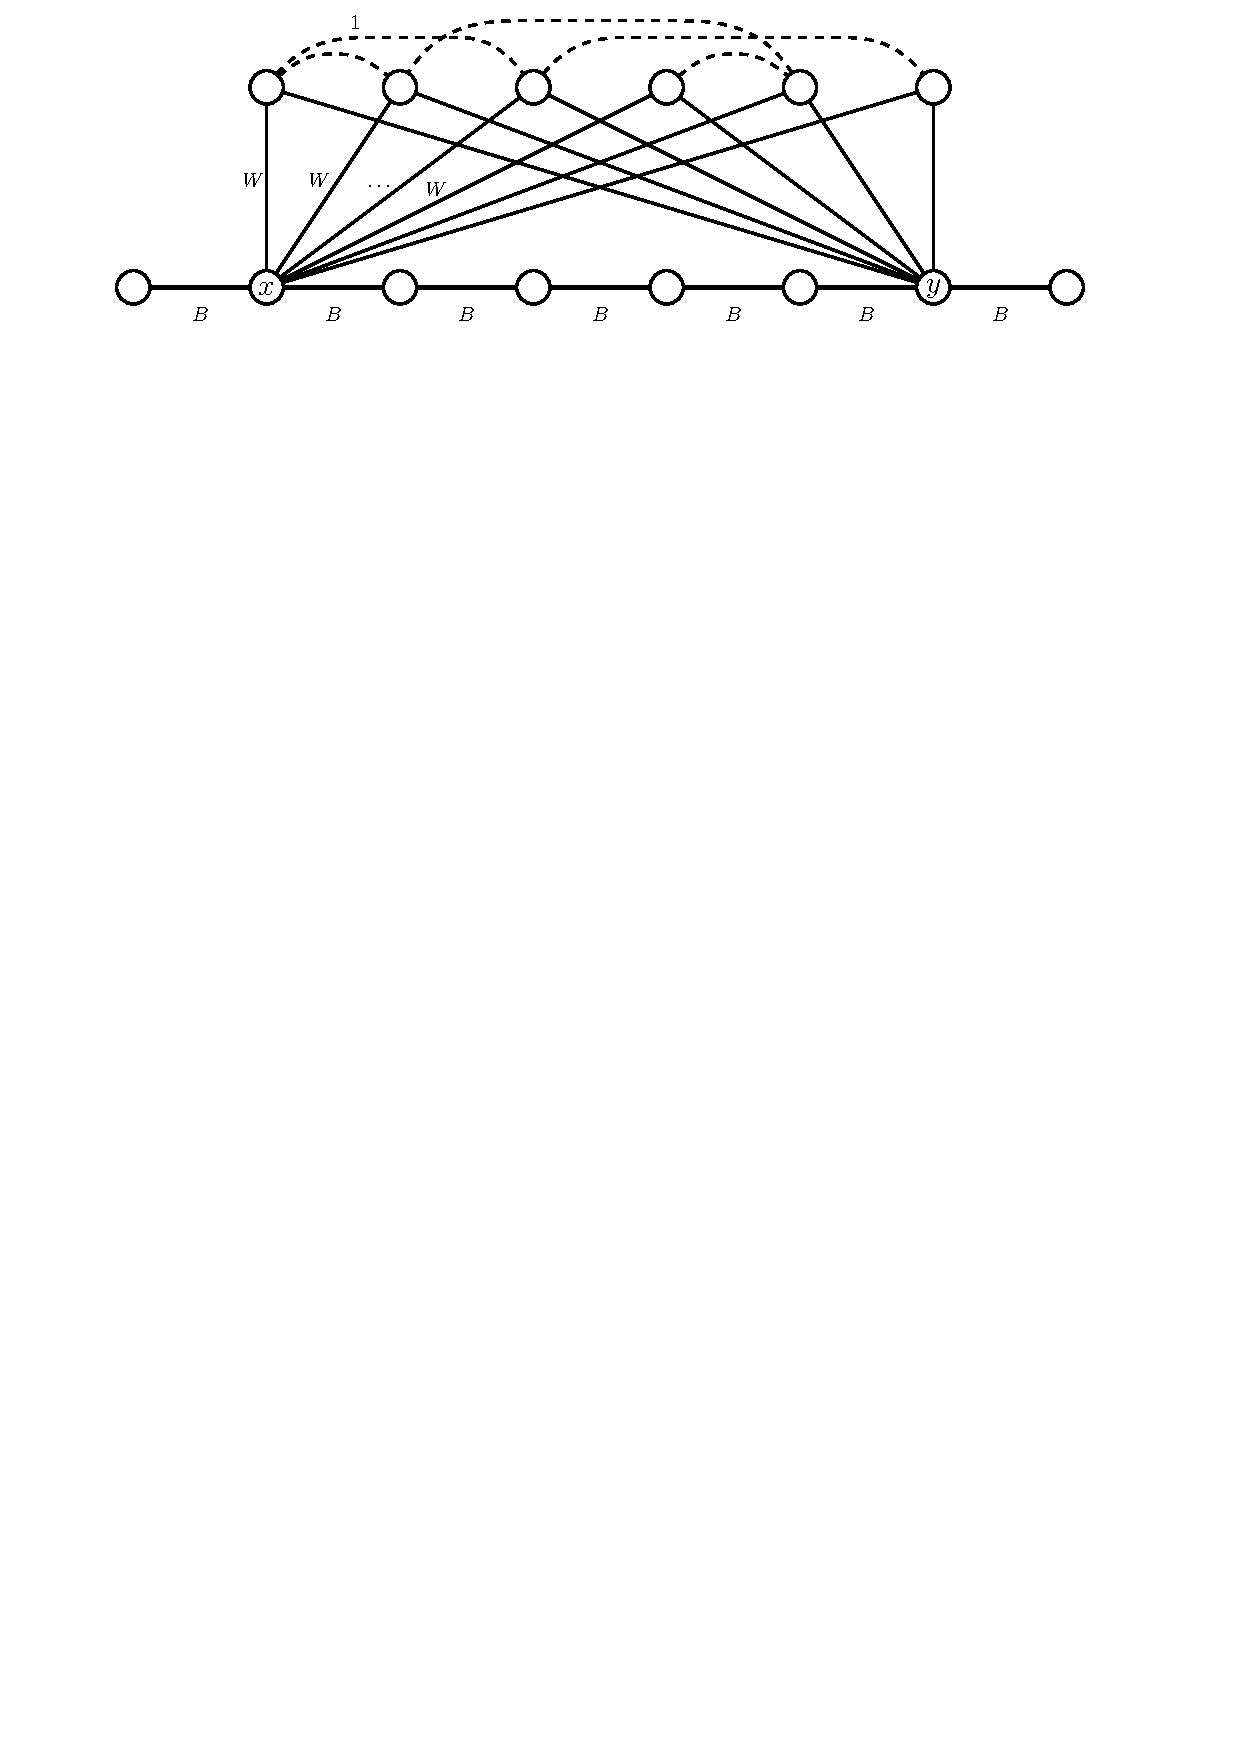
\includegraphics[width=0.3\textwidth]{figs/substitute}
%	\caption{Cluster types used in the analysis of \TAlg.}
%\end{figure}

In our analysis, we distinguish among three types of clusters: $C_1, C_2, C_3$. In a cluster of type $C_i$, the size of the largest component contained in this cluster is $i$.
Before bounding the competitive ratio of \TAlg, we introduce the lemma that upper bounds the cost of a single repartition of \TAlg.

\begin{lemma}
	\label{lem:1req}
	In a single reconfiguration of nodes (after a merge of components), \TAlg exchanges at most $2$ pairs of nodes.
\end{lemma}

\begin{proof}
	Observe that when the repartition is triggered by \TAlg, the resulting partitioning is component respecting.
	Otherwise, if it does not exist, \TAlg simply ends the phase and performs no repartition.
	
	%We distinguish between three types of clusters: $C_1, C_2, C_3$,
	%which we define as follows.
	%A cluster of type $C_1$ the cluster contains $3$ singleton components (this is also the initial configuration of any cluster).
	%A cluster of type $C_2$  contains one component of size $2$ and one component of size $1$.
	%Finally, a cluster of type $C_3$  contains one component of size $3$.
	
	Consider a request between $u$ and $v$ that triggered the repartition and let $U$ and $V$ be their respective clusters.
	The request triggered the repartition, hence it was external and $U\neq V$.
	We consider cases based on the types of clusters $U$ and $V$.
	
	If either $U$ or $V$ is of type $C_1$, then this cluster can fit the merged component, and the reconfiguration is local within $U$ and $V$.
	In this case, a local repartition is possible (within $U$ and $V$), for a cost of at most $2$ swaps.
	Note that it is impossible that either $U$ or $V$ is of type $C_3$, as otherwise, a components of size $3$ participates in a merge.
	After merge, we would have a component of size at least $4$, and in this case no component respecting partitioning exists, a contradiction.
	
	
	It remains to consider the case where both $U$ and $V$ are of type $C_2$. Note that $(u,v)$ cannot both belong to a component of size $2$, as this would mean that \TAlg has the component of size $4$, a contradiction with the case assumption that the component respecting partitioning exists. 
	Otherwise, if either $u$ or $v$ belongs to a component of size $2$, then it suffices to exchange components of size $1$ between $U$ and $V$.
	Finally, if $u$ and $v$ belong to components of size $1$, then we must place them in a cluster different from $U$ and $V$.
	Note that in such case, a $C_1$-type cluster $W$ exists, as otherwise no component respecting partitioning exists. In this case \TAlg performs one swap, i.e., it exchanges the nodes $u$ and $v$ with any two nodes of $W$.
\end{proof}



\begin{figure}[H]
	\centering
	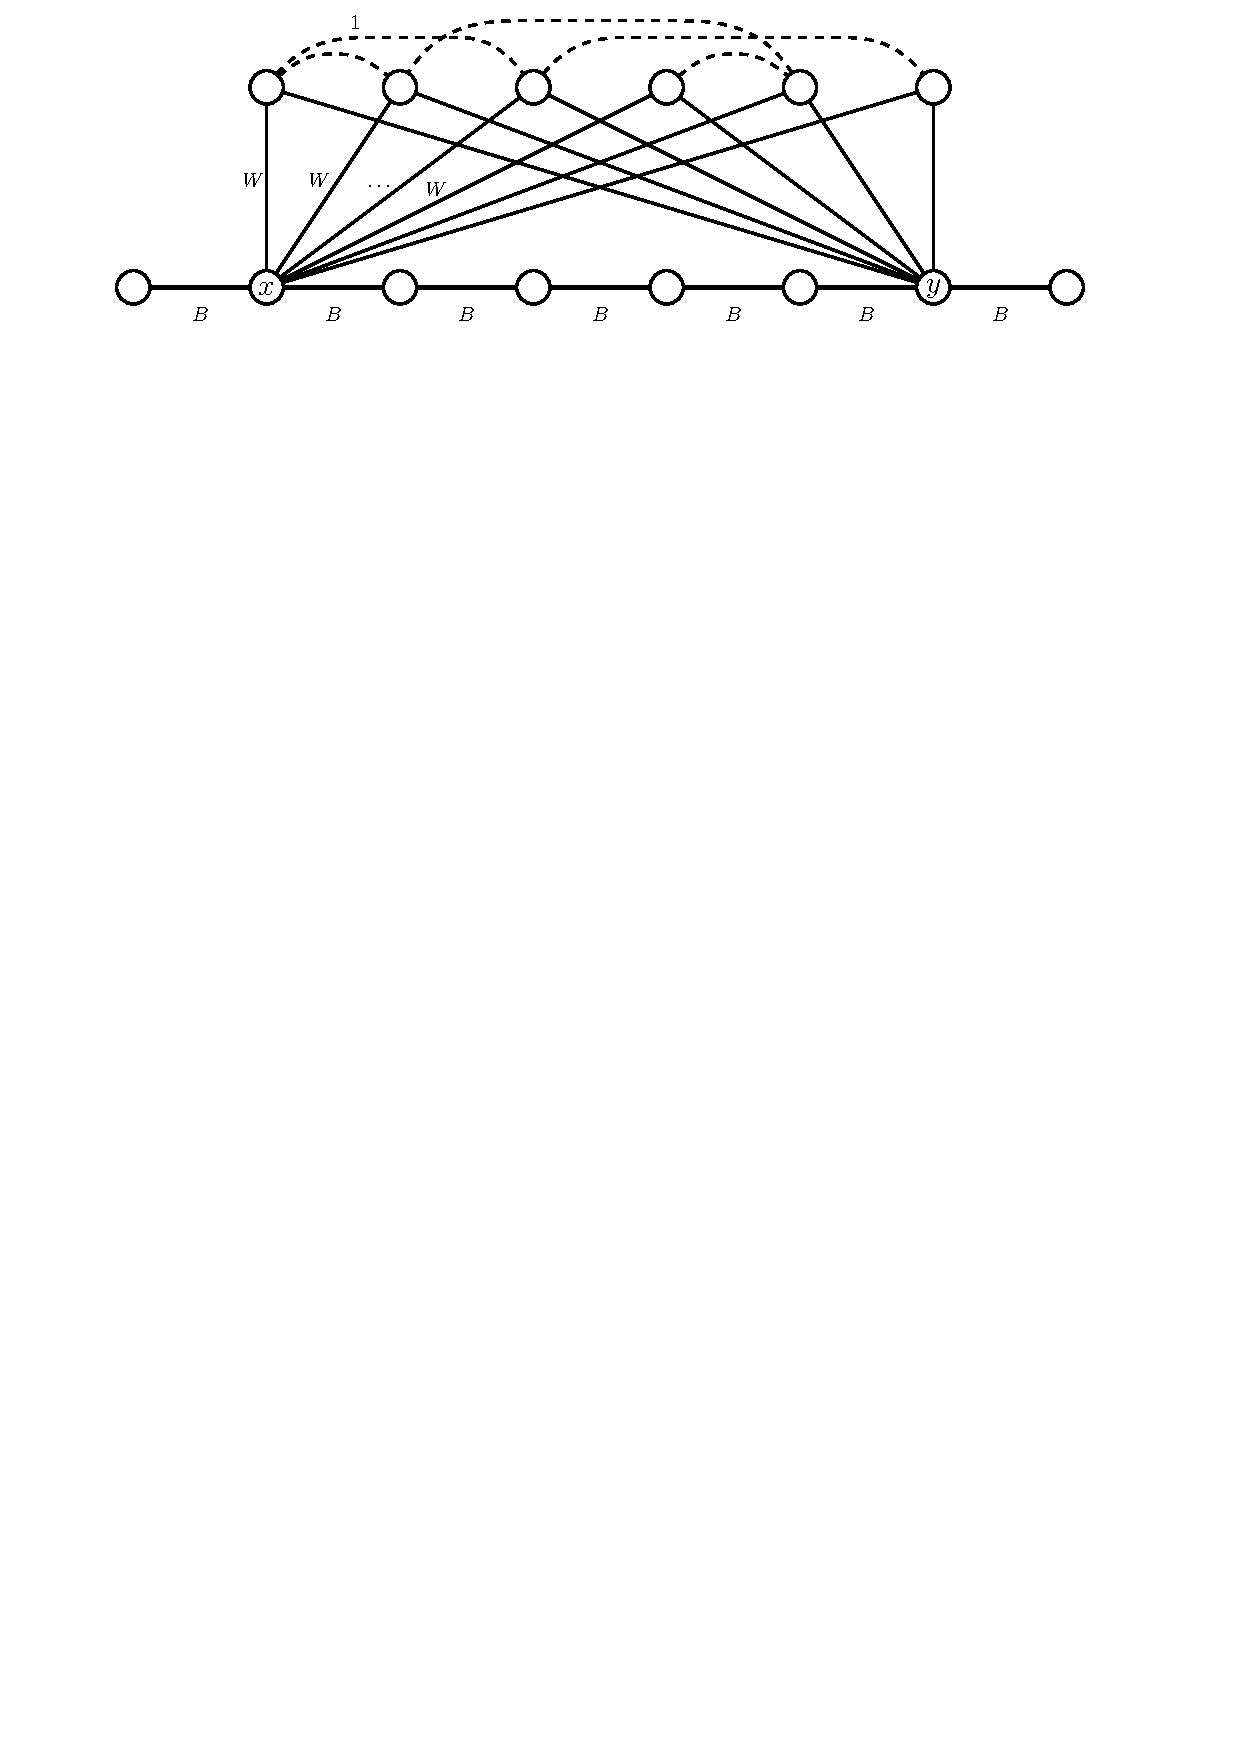
\includegraphics[width=0.3\textwidth]{figs/substitute}
	\caption{an unsaturated edge that is inside a component. If there is a space next to it, maybe cluster types should fit next to it? Not sure.}
\end{figure}



\begin{theorem}
	\TAlg is $(54\ell)$-competitive for $k=3$.
\end{theorem}
\begin{proof}
	Fix a completed phase, and consider the state of \TAlg's counters at the end of it.
	We consider the incomplete phase later in this proof.
	
	As \TAlg is component respecting, it never increases any counter above $\alpha$.
	We say that the pair $(u, v)$ is \emph{saturated} if the counter has value $\alpha$, and \emph{unsaturated} otherwise.
	By $\sigma$ we denote the input sequence that arrived during the phase.
	By $\sigma_{cost}$ we denote the requests that at the moment of arrival were external requests for \TAlg (these are the only requests that incur cost for \TAlg).
	In our analysis, we partition $\sigma_{cost}$ into subsequences $\sigma_I$ and $\sigma_E$.
	The sequence $\sigma_I$ (inter-component requests) are the requests from $\sigma_{cost}$ issued to pairs that belong to the same component of \TAlg at the end of the phase.
	The sequence $\sigma_E$ (extra-component requests) denotes the requests from $\sigma_{cost}$ that do not appear in $\sigma_I$.
	
	
	%Let $A^I$ be the cost of (extra-cluster) communication incurred in this phase by \TAlg between pairs that belonged to the single component at the end of the phase.
	%Let $A^E$ be the cost of (extra-cluster) communication incurred in this phase between the nodes that belong to different components at the end of this phase.
	Let $\TAlg(M)$ be the cost of migrations performed by \TAlg in this phase.
	\TAlg performs at most $2 \ell$ component merge operations, as
	exceeding this number means that a component of size $4$ exists, and the phase should have ended already.
	Combining this with Lemma~\ref{lem:1req} gives us $\TAlg(M) \leq 8\alpha\cdot\ell$ (recall that an exchange costs $2\alpha$).
	%Together with Lemma~\ref{lem:1req}, this allows us to bound the cost of migrations, $\TAlg(M) \leq 6\cdot\alpha\cdot\ell$.
	
	Now we bound $\TAlg(\sigma_I)$.
	A~cluster of type $C_3$ contributes at most $3 \alpha - 1$ to $\TAlg(\sigma_I)$, as two pairs of nodes from the component are saturated and contribute $\alpha$ each, and the third, unsaturated pair contributes at most $\alpha-1$.
	Other cluster types contribute less: $C_1$ contributes~$0$ and $C_2$ contributes $\alpha$.
	Summing this over all $\ell$ clusters gives us $\TAlg(\sigma_I) \leq (3 \alpha-1)\cdot \ell \leq 3\alpha\cdot\ell$.
	
	%We bound $A^E$ by $k^2 \cdot (\alpha - 1)$, as no more than $k^2$ pairs are unsaturated, and each of them contributes at most $\alpha -1$.
	%\maciek{not needed most likely}
	
	Moreover, \TAlg paid for all requests from $\sigma_E$, and thus $\TAlg(\sigma_E) = |\sigma_E|$.
	In total, the cost of \TAlg is at most $\TAlg(\sigma_I) + \TAlg(\sigma_E) + \TAlg(M) \leq 11\alpha\cdot \ell + |\sigma_E|$ during this phase.
	
	\medskip
	
	Now we lower-bound the cost of $\OPT$.
	By $\OPT(\sigma_I)$ and $\OPT(\sigma_E)$ we denote the cost of $\OPT$ on requests from sequences $\sigma_I$ and $\sigma_E$, respectively.
	Note that these costs are defined with respect to components of \TAlg in this phase.
	By $\OPT(M)$ we denote the cost of migrations performed by $\OPT$ in this phase.
	
	We split the cost of $\OPT$ into parts coming from serving $\sigma_I$ and $\sigma_E$.
	While serving these requests, $\OPT$ may perform migrations, and we account for them in both parts: we separately bound $\OPT$ by $\OPT(\sigma_I) + \OPT(M)$ and $\OPT(\sigma_E) + \OPT(M)$.
	Combining those bounds gives us $\OPT \geq \max\{\OPT(\sigma_I) + \OPT(M), \OPT(\sigma_E) + \OPT(M)\} \geq (\OPT(\sigma_I) + \OPT(M)) / 2 + (\OPT(\sigma_E) + \OPT(M)) / 2$.
	
	%Let $O^M$ be the cost of migrations performed by $\OPT$ during the phase.
	%Let $O^I$ be the cost of serving requests between nodes that were put in one component by \TAlg during this phase.
	%Let $O^E$ be the cost serving requests between nodes that \TAlg did not put in the same component during that phase.
	
	%First, we estimate the cost related to $\sigma_I$.
	We have $\OPT(M) + \OPT(\sigma_I) \geq \alpha$, as the phase ended when the components of \TAlg{} could not be partitioned without splitting them.
	Hence, for every possible configuration of $\OPT$, there exists a non-collocated pair of nodes with at least $\alpha$ requests between them, and
	$\OPT$ either served them remotely or performed a~migration.
	
	\medskip
	Before we bound the competitive ratio, we relate the costs of $\TAlg$ and $\OPT$ with respect to requests $\sigma_E$.
	By entering some fixed configuration before serving $\sigma_E$, \OPT may mitigate paying for requests between at most $3\ell$ pairs of nodes by collocating them in its clusters.
	Recall that $\sigma_E$ consists of requests to unsaturated pairs, and it accounts only for requests that increased the counter (i.e., external requests), thus $\OPT$ may mitigate at most $3\ell\cdot(\alpha - 1)$ requests from $\sigma_E$.
	Faced with at least $W := |\sigma_E| - 3\ell\cdot(\alpha-1)$ requests $\sigma_E$ that it could not mitigate, $\OPT$ served some of them remotely and possibly performed some migrations to decrease its cost.
	
	
	Now we estimate the cost of $\OPT(\sigma_E)$ while accounting savings from migrations.
	By performing a swap of nodes $(u,v)$, $\OPT$ collocates $u$ with two nodes $u', u''$, and $v$ with two nodes $v'$, $v''$.
	This may allow serving requests between $(u,u')$, $(u,u'')$, $(v,v')$ and $(v,v'')$ for free afterwards.
	As $\sigma_E$ consists of requests to unsaturated pairs, and it accounts only for external requests, there are at most $\alpha-1$ requests between each of these pairs.
	By performing a single swap that costs $2\alpha$, $\OPT$ may avoid paying the remote serving costs for at most $4 (\alpha - 1)$ requests from $\sigma_E$
	Hence, for serving $\sigma_E$, $\OPT$ pays at least $\OPT(\sigma_E) + \OPT(M) \geq W \cdot \frac{2\alpha}{4 (\alpha-1)}\geq |\sigma_E| / 2 - 2 \alpha \cdot \ell$.

	
	Finally, we bound the competitive ratio.
	From the bound on \OPT's cost we have $|\sigma_E| \geq 2(\OPT(\sigma_E)+\OPT(M)) + 4\alpha \cdot \ell$.
	Let $\xi := \OPT(\sigma_E) + \OPT(M)$.
	The competitive ratio is

	\[
		\frac{\TAlg(\sigma)}{\OPT(\sigma)} \leq \frac{11\alpha \cdot \ell + |\sigma_E|}{\alpha/2 + \xi/2} \leq \frac{27\alpha\cdot\ell + 2\cdot \xi}{\alpha + \xi} \leq 27 \ell.
	\]
	
	\medskip
	
	It remains to consider the last, unfinished phase.
	First, consider the case, where the unfinished phase is also the first one.
	Then, we cannot charge $\OPT$ due to the inability to partition the components.
	Instead, we use the fact that \TAlg and $\OPT$ started with the same initial configuration.
	If the input finished before the first $\alpha$ external requests, then \TAlg is $1$-competitive.
	If there were at least $\alpha$ external requests, then $\OPT$ either paid $\alpha$ for serving them remotely, or paid $\alpha$ for a migration; for the cost of \TAlg we follow the analysis of the unsaturated pairs.
	Second, consider the case, where there are at least two phases, then we split the cost $\alpha$ charged in the penultimate phase into last two phases, and follow the analysis regarding the unsaturated requests.
	This way, the competitive ratio increases at most twofold in comparison to a finished phase, and the competitive ratio is $\TAlg(\sigma)/\OPT(\sigma) \leq 54\ell$.
\end{proof}

\subsection{Improved algorithm for Online Rematching} \label{sec:k2}
In this section,
we present \RM,
 an algorithm for the \OBRP restricted to clusters of capacity $k=2$.
We interpret a pair of nodes collocated in one cluster as a matched pair.
Hence,
the problem is an online variant of the classic matching problem where
a matched pair can separate from each other in order to ``rematch'' with two other nodes.
This is known as the  \emph{Online Rematching} 
problem and a (non-strict) 7-competitive algorithm is already given by \cite{repartition-disc},
in which the ratio comes with an additive factor in $O(\alpha\ell^2)$.
We do not only improve upon their competitive ratio,
but also show that our ratio holds \emph{strictly}
(i.e., with no additive factor).
In addition,
our algorithm is similar
and slightly simpler than the one in \cite{repartition-disc}, 
while our analysis is significantly more simple and concise,
thanks to the charging scheme we devise here.


We describe the algorithm \RM for the online rematching problem as follows.
The input to \RM is a sequence of  requests
$\sigma:=\{\sigma_1,\dots, \sigma_m\}, \sigma_t:=\{x,y\} \in V^2, x \neq y$.
We maintain a counter $C_{\set{x,y}}$ for each pair of nodes $\set{x,y}$ and increment it on every remote request between $x$ and $y$.
Once $C_{\set{x,y}} = \lambda$,
reset the counter and collocate the pair arbitrarily in one of the two clusters where $x$ or $y$ resides.

\begin{theorem} \label{thm:k=2}
	The algorithm \RM, for $\lambda=\alpha$, is (strictly) 6-competitive.
\end{theorem}


We charge both \OPT and \RM whenever \RM collocates a pair (i.e., on a collocation event).
%More precisely,we charge them only the cost of the collocation, per such event.
%Hence,we charge the cost of  this collocation to \OPT for the first time.
\RM collocates a pair always with a swap (i.e., two simultaneous migrations),
which  costs $2\alpha$,
while OPT may save some costs by collocating multiple pairs at once, 
 before they inflict too much communication cost.
 Therefore it pays the price of only one migration per pair  (\mahmoud{see Figure \ref{fig:TBD}}).
Hence,
whenever \OPT collocates a pair,
we charge it only the cost of moving a single node to the cluster of the other,
i.e., $\alpha$ (in contrast to $2\alpha$ on \RM).

\textbf{The charging scheme.}
Consider two  pairs that share a same node, 
i.e.~\emph{intersecting pairs},
and the set of requests that causes the collocation of both pairs,
at some  times during  $[1,m]$.
%i.e.~the entire duration of the sequence.
Observe that \OPT must pay a non-zero cost
for these requests over the entire $\sigma$,
since it cannot have both pairs initially collocated.
However,
we can charge the whole cost to \OPT only the first time \RM collocates a pair,
and not at any consequent time when \RM collocates it a second time.
Otherwise,
 \OPT is possibly charged for a same cost repeatedly.
For this reason,
we charge \OPT a cost inflicted by a pair,
if and only if  \OPT incurs the cost some time since the last time \RM separated the pair.
%%

\begin{proof}[Proof of Theorem \ref{thm:k=2}]
	Assume on request $\sigma_{t}=\set{u,v}$, 
	i.e., at (time) $t$,
	\RM collocates the pair $\set{u,v}$.
	This means,
	the value of $C_{\set{u,v}}$ at $t$,
	denoted by $C^t_{\set{u,v}}$, 
	reaches $\lambda$ immediately before \RM resets the counter.
	I.e.,
	$ C^t_{\set{u,v}} = \lambda$.
	We denote the set of all requests to a pair $\set{x,y}$ that arrive
	during $[t_1,t_2]$ by $\sigma_{\set{x,y}}[t_1,t_2]$,
	and its overall cost to \OPT by
	$\mathit{OPT} (\sigma_{\{u,v\}}[t_1,t_2])$.
	We may use $\sigma_{\set{x,y}}$ whenever
	 the interval $[t_1,t_2]$ is clear from the context.
	%
	%Else, this is not the first time and
	%Alg collocates $\{u,v\}$ also some time prior to $t$.
	
	If $t$ is not the first time that \RM collocates $\{u,v\}$ then
	let $0 < t' < t$ be the latest time when \RM separates $\set{u,v}$
	in order to collocate some intersecting pair
	$\{x,y\} \neq \{u,v\}, \{x,y\} \cap \{u,v\} \neq \emptyset$, 
	e.g.,
	$\{x,y\}=\{u,w\}$.
	Else,
	$t$ is the first time that \RM collocates $\{u,v\}$ and let $t' := 0$.
	Similarly,
	if $t' > 0$ is not the first time that \RM  collocates $\{u,w\}$ 
	then let $0 < t'' < t'$ be the latest time before $t'$ when \RM separates $\set{u,w}$.
	Else,
	$t'$ is the first time that \RM collocates $\{u,w\}$ and we let $t''=0$.
	%
	
	First,
	we bound  costs incurred by \RM for requests that
	lead to the collocation of $\{u,v\}$ at time $t \in T$, where
	$T := \{ i \in [1,m] ~\vert~ \exists \{x,y\}: C^{i}_{\{x,y\}} = \lambda \}$
	is the set of times when \RM performs a collocation.
	By definitions of $t$ and $t'$,
	the overall cost of requests in $\sigma_{\set{u,v}}$ incurred by \RM,
	i.e., the total cost of remote serving
	and the moving cost, is
	$\lambda + 2\alpha$.	
	Next,
	we bound costs incurred by \RM
	for requests that do not lead to collocations until the  end of the sequence at $t=m$.
	Assume $\{u,v\}$ is not collocated at $t=m$
	and $0 < C^{m}_{ \{u,v\} } < \lambda $,
	which means \RM pays $C^{m}_{ \{u,v\} }$
	for  requests in $\sigma_{\set{u,v}}(t',m]$.
    Then the overall cost to \RM is
$	\mathit{RM} (\sigma)
=
\sum_{ t \in T}(\lambda + 2\alpha) +
\sum_{\{u,v\}} C^{m}_{\{u,v\}}	
$.
	
	Next,
	we bound  costs incurred by \OPT for requests that trigger collocation of $\{u,v\}$ at $t \in T$.
	If $t$ is the first time that \RM collocates $\{u,v\}$ then  \OPT pays
	$\lambda$ for serving requests in $\sigma_{\set{u,v}}[0,t]$ (remotely),
	or $\alpha$ for collocating the pair and
	serving (some of) the requests with  cost zero.
	Therefore in this case,
	$\OPTM (\sigma_{\{u,v\}}(0,t]) \geq  \min{\{ \lambda,\alpha \}}$.
	%
	Otherwise,
	it is not the first collocation and
	consider times $t'$ and $t''$ as define previously,
	 and let 
	$R_t := \sigma_{\{u,w\}}(t'',t'] \cup \sigma_{\{u,v\}}(t',t] $.
	We define $R_{t'}$ for the collocation at $t'$  analogously.
	Then,
	$\OPTM(R_t) = \mathit{OPT} (\sigma_{\{u,w\}}) 
	+ \OPTM(\sigma_{\{u,v\}}) $.
	Note that \OPT cannot have both pairs collocated at the same time.
	However, it can have one of the pairs already collocated prior to its respective interval.
	Let us assume  \OPT has one pair,
	e.g.~$\{u,v\}$ collocated already prior its respective interval, i.e.~$(t',t]$,
	 and keeps it so during the interval.
	 Then it pays zero while serving $\sigma_{\{u,v\}}$.
	Hence,
	it must pay $\alpha$ for collocating the other pair, in this case $\{u,w\}$,
	or (resp., and) it pays (resp., up to) $\lambda$ for serving (resp., some of) requests in $\sigma_{\{u,w\}}$. 
	Therefore in any case,
	$\OPTM(R_t) \geq  \min{\{ \lambda,\alpha \}}$.
	
	It remains to bound the cost  incurred by \OPT due to requests to $\{u,v\}$ that do not lead to its collocation until the end of the sequence at $t=m$.
	We bound the cost analogously to the case where \RM collocates $\{u,v\}$.
	If $\{u,v\}$ is not collocated in the initial matching
	and \RM never collocates it,
	then $ C^{m}_{ \{u,v\} } =| \sigma_{\{u,v\}}[1,m] |$.
	\OPT pays
	$\mathit{OPT} (\sigma_{\{u,v\}}[1,m]) 
	\geq \min{ \{ \alpha, C^{m}_{ \{u,v\} } \} }$,
	for collocating this pair or (and) paying for (resp.~some of) requests in $\sigma_{\{u,v\}}[1,m]$.
	Else,
	either $\{u,v\}$ is collocated in the initial matching
	or \RM collocates it at some point.
	Then there exists an intersecting pair $\set{u,w}$
	that is collocated by \RM at $t' < m$,
	separating $\{u,v\}$.
	We define times $t'' < t' < m$ similarly as in the former case.
	Let $R^*_{\{u,v\}} := \sigma_{\{u,w\}} (t'',t'] \cup \sigma_{\{u,v\}} (t',m]$.
	Then,
	\OPT must pay for collocating at least one pair or (and) serving requests 
	to the other pair remotely.
	Thus,
	$\mathit{OPT} (R^*_{\{u,v\}}) 
	\geq  \min{ \{ C^{m}_{ \{u,v\}}, \alpha \}}$.
	
	Next, we sum up all costs incurred by \OPT.
	By definitions of $R_t$ and $R^*_{\{u,v\}}$, we have either
	$R_{t'} \cap R_t = \sigma_{\{u,w\}}$ or
	$R_{t'} \cap R^*_{\{u,v\}} = \sigma_{\{u,w\}}$
	(\mahmoud{See figure \ref{fig:doubleCount}}). 
	This means,
	$\OPTM ( \sigma_{\{u,w\}})$
	is counted at most twice in each of  the expressions
	$\mathit{OPT} (R_{t'}) + \mathit{OPT} (R_t)$
	and  
	$\mathit{OPT} (R_{t'}) + \mathit{OPT} (R^*_{\{u,v\}})$.
	Hence,
	for all collocations performed by \RM,
	and for final costs at $t=m$,
	\OPT pays at least 
	$\frac{1}{2}(
	\sum_{ t \in T } \mathit{OPT} (R_t) +
	\sum_{\{u,v\}} \mathit{OPT} (R^*_{\{u,v\}})
	) $.
	Then,
	the total cost to \OPT is
	
	\begin{align*} 	%\label{eq:costOPT}
		\mathit{OPT} (\sigma)
		&=
		\frac{1}{2}
		\Big(
		\sum_{ t \in T} \mathit{OPT} (R_t) 
		+ \sum_{\{u,v\}}\mathit{OPT} (R^*_{\{u,v\}})
		\Big)	\\
		&\geq
		\Big(
		\sum_{ t \in T} \min{ \{ \lambda, \alpha \}}  +
		\sum_{\{u,v\}} \min{ \{C^{m}_{\{u,v\}} , \alpha \} } 
		\Big)		
		=
		\frac{1}{2}		
		\Big(
		\sum_{ t \in T} \alpha  
		+ \sum_{\{u,v\}} C^{m}_{\{u,v\}}
		\Big).
	\end{align*}

Finally, we have

\begin{align*}
	\mathit{ALG} (\sigma)	/
	\mathit{OPT} (\sigma)
	\leq
	2\Big(
	\sum_{ t \in T} 3\alpha +
	\sum_{\{u,v\}} C^{m}_{\{u,v\}}
	\Big)	 \big /
	\Big(
	\sum_{ t \in T} \alpha  
	+ \sum_{\{u,v\}} C^{m}_{\{u,v\}}  
	\Big)	\leq 6.
\end{align*}
%	The claim follows from here.

\end{proof}

\section{Discussion and Future Work}

\mahmoud{mention the offline approx.}
While we have described our algorithms globally so far, we note that these allow for efficient distributed implementations. 
The algorithm PPL from Section~\ref{sec:ppl} can be distributed
similarly to the approach in~\cite{sigmetrics19_partitioning}.
The algorithm for $k=2$ from Section~\ref{sec:k2} performs only local communication for each request: counters are kept on the clusters and updated locally, and each migration concerns only two clusters.
\medskip
Now, we propose the distributed implementation of the algorithm for $k=3$ from Section~\ref{sec:k3}.
The algorithm performs two non-local operations:
\begin{enumerate}
	\item Broadcasting the end of the phase.\label{it:broadcast}
	\item Component merge.
	\label{it:merge}
\end{enumerate}

If a component reaches size $4$ or a fresh cluster is not found, we conclude that no perfect partition exists.
Then, we end the phase and broadcast the message to  reset the counters in all clusters.

A merge of two components may require finding a third cluster that contains $3$ isolated nodes (for details see the proof of Lemma~\ref{lem:1req})).
We say that a cluster containing $3$ isolated nodes is \emph{fresh}.
In the following, we show how to efficiently find a fresh cluster in a distributed manner.
We organize the clusters into an arbitrary rooted balanced binary tree, and we broadcast the root to each cluster.
Each cluster maintains the counter of fresh clusters in its subtree.
To find a fresh cluster, we traverse an arbitrary path of non-zero counters from the root.
Upon encountering a fresh cluster, we stop the traversal and decrease the counters on the followed path by $1$.

The operation (\ref{it:broadcast}) requires a single broadcast, and the operation (\ref{it:merge}) requires $O(\log \ell)$ communication.
Each of these may occur, on average, every $\alpha$ external requests.

\medskip

This paper revisited the dynamic graph partitioning problem and presented several tight bounds for the important model where capacities cannot be exceeded, both for a general partitioning model and for a special learning model. 

While are bounds are tight, there are several interesting avenues for future research.
In particular, we have so far focused on deterministic algorithms, and it would be interesting to study the power of randomization in this context.
On the practical side, it would also be interesting to study our algorithms empirically, under realistic workloads.

\bibliographystyle{plainurl}
\bibliography{references}
\appendix


\end{document}
